\documentclass[]{article}
\usepackage[utf8]{inputenc} % UTF8 юникод текст оруулах
\usepackage[T2A]{fontenc} % кирил үсгийн кодчилол
\usepackage[mongolian]{babel} % олон хэлний текст
\usepackage{graphicx}
\graphicspath{ {images/} }
\title{Хэрэглэгчийн профайл}
\author{Ч.Анударь B140920739}


\begin{document}
	\maketitle
	
	\newpage
	\section{Шинжилгээ, зохиомжийн хэсэг}
	\subsection{Функциональ шаардлага}
	\begin{itemize}
		\item Өөрийн хувийн мэдээлэлээ оруулна  (сурдаг сургууль, оршин суудаг газар,онцолсон зургуудаа нэмэх )
		\item Вэбсайт дээрх өөрийн үйл ажилагааг харах (Дараах хэрэглэгчид харагдах байдал, Цагийн хүрдний тохиргоо)
		\item Өөрийн бүхий л мэдээллийг харж солиж устгаж мэдээлэл нэмэх 
		\item Хэрэглэгч зураг эсвэл бичлэг нийтэд нийтлэл
		\item Хэрэглэгч өөрт ирсэн найз болох хүсэлтийг жагсаалтаар харах найз болон хүсэлтүүдийг харна шинээр найз нэмнэ бас хасаж болно
		\item Хэрэглэгч нийтлэл, грүпп эсвэл өөр бусад хэрэглэгчийг хайх
		\item Хэрэглэгч өөрийн мэдээлэл болон бусад тохиргоох харуулах
	\end{itemize}
	\section{Функциональ бус шаардлага}
	\begin{itemize}
		\item Түргэн шуурхай ажиллах
		\item Энгийн бөгөөд ойлгомжтой 
		\item Алдааны мэдээлэл өгдөг байх 
		\item Бүх төрлийн төхөөрөмжид тохиромтой хэлбэрээр харагддаг /респонсив/ загвартай байна.
	\end{itemize}
\subsection{Use-case diagram}
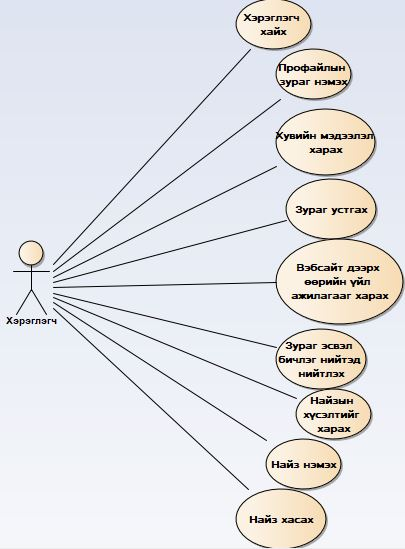
\includegraphics[width=\textwidth]{usecaseZ}
\subsection{Дэлгэц}
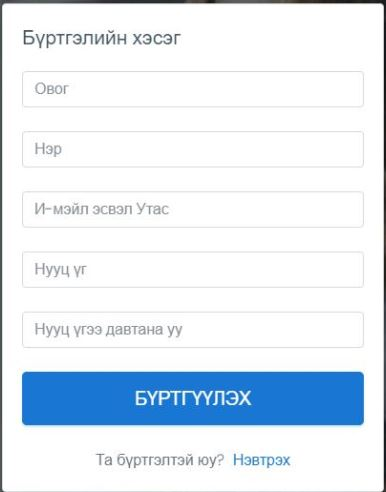
\includegraphics[width=\textwidth]{delgets}
\subsection{Зураг оруулах activity}
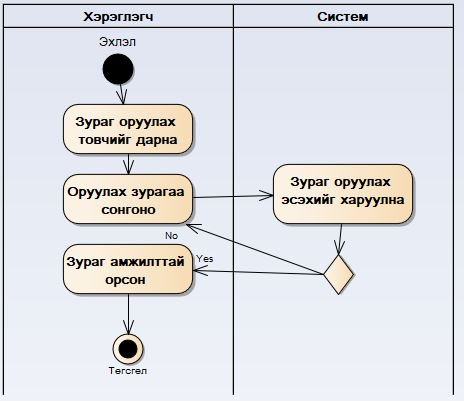
\includegraphics[width=\textwidth]{activity1}
\subsection{Найзын хүсэлтийн activity}
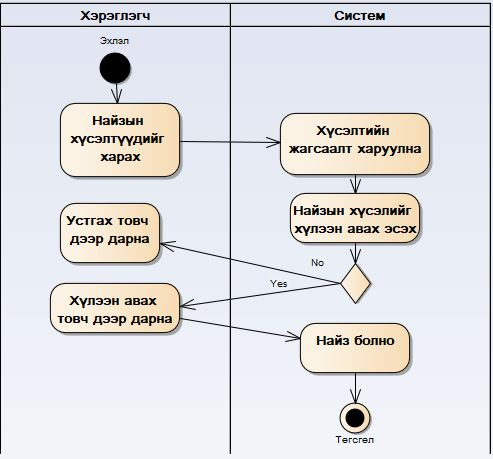
\includegraphics[width=\textwidth]{activity2}
\subsection{Обьект холбоосын диаграм (ERD)}
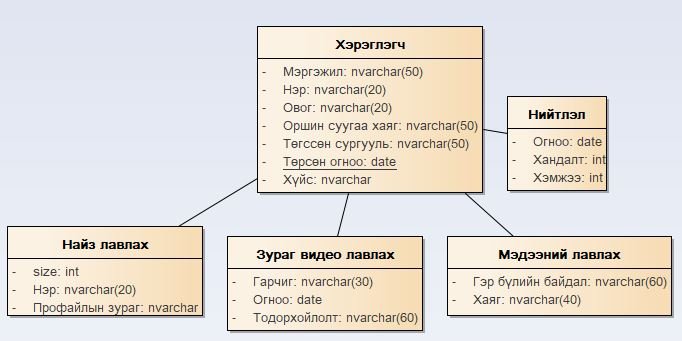
\includegraphics[width=\textwidth]{ERD}
\subsection{Класс диаграм (Class diagram)}
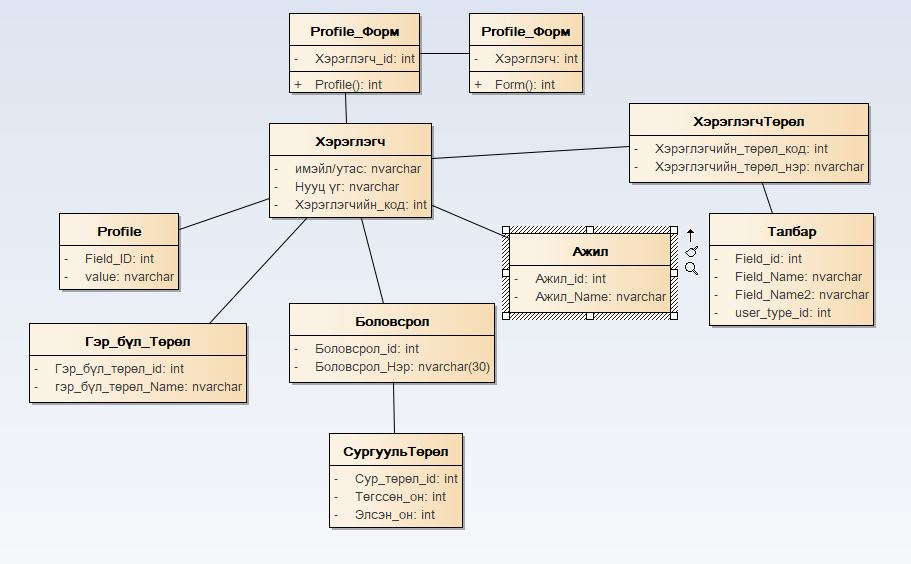
\includegraphics[width=\textwidth]{CLASS}
\subsection{Класс диаграм (Sequence diagram)}
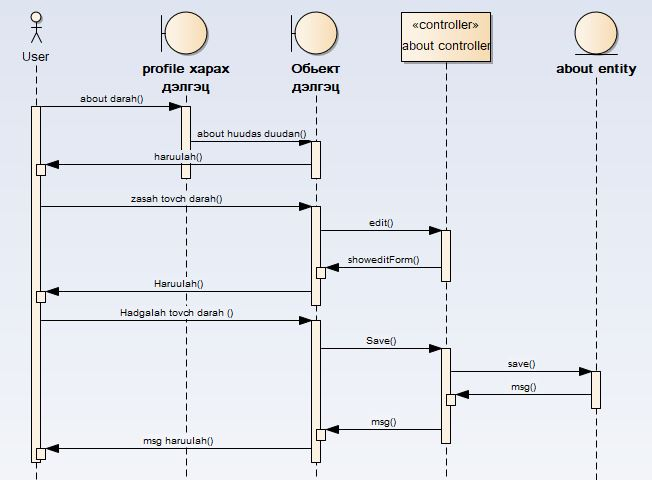
\includegraphics[width=\textwidth]{seq1}
\end{document}
